

\documentclass[aps,prb,twocolumn,groupedaddress,10pt,longbibliography,nofootinbib]{revtex4-2}
\usepackage{graphicx}
\usepackage{amsmath}
\usepackage{amssymb}
\usepackage{color}
\usepackage{ulem}
\usepackage[pdfstartview=FitH]{hyperref}
\pdfminorversion=7

\begin{document}

\title{Star Wars Episode IV: A New Hope}

\author{O.-W. Kenobi}

\affiliation{Tatooine, A Galaxy Far, Far Away.}

\begin{abstract}
It is a period of civil war. Rebel spaceships, striking from a hidden base, have won their first victory against the evil Galactic Empire. During the battle, Rebel spies managed to steal secret plans to the Empire’s ultimate weapon, the DEATH STAR, an armored space station with enough power to destroy an entire planet. Pursued by the Empire’s sinister agents, Princess Leia races home aboard her starship, custodian of the stolen plans that can save her people and restore freedom to the galaxy….
\end{abstract}

\maketitle

\section{Introduction}

Bobrick \textit{et al.} recently proposed a physical model for a warp drive\cite{Bobrick_2021}. The experiment proposed in ref.~\cite{PhysRevLett.128.163603} could finally show us what hyperspace looks like.

According to Einstein's theory of special relativity, energy is given by
\begin{equation}
E^2=(pc)^2+(mc^2)^2
\label{eq:Esquared}
\end{equation}

The Imperial Death Star, shown in fig.~\ref{fig:death_star}, generates enough energy to destroy an entire planet.
\begin{figure}%
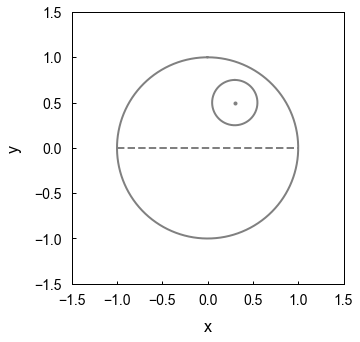
\includegraphics[width=\columnwidth]{deathstarfig}%
\caption{The Death Star.}%
\label{fig:death_star}%
\end{figure}

The Death Star is estimated to have a diameter of around 160 km, housing nearly 2 million personnel. A breakdown is shown in table~\ref{table:forces}.
\begin{table}%
\begin{tabular}{|l|l|}
\hline
Crew & 265,675 \\
Troops & 607,360\\
Stormtroopers & 30,984\\
Gunners & 52,276\\
Pilots & 180,216\\
Support & 42,782\\
\hline
\end{tabular}
\caption{Death Star Personnel}
\label{table:forces}
\end{table}

The Death Star has only one vulnerability -- a thermal exhaust port just below the main port that leads to the main reactor. It is believed that a proton torpedo fired into the port will set off a chain reaction sufficient to destroy the space station. The target area is only two metres wide but is within the accuracy of the targeting system of the Rebel Alliance's X-wing fighters.

\textcolor{red}{This text is red.}
\sout{This is strikethrough text.}

\begin{acknowledgments}
The author acknowledges helpful discussions with L. Skywalker and H. Solo. This work was funded by the Rebel Alliance.
\end{acknowledgments}



\bibliography{references}

\end{document}